\documentclass[runningheads]{llncs}
\usepackage{graphicx}
\usepackage{float}
\restylefloat{figure}
\usepackage{xcolor}
\usepackage{listings}
\lstset{
  language=C,                % choose the language of the code
  numbers=left,                   % where to put the line-numbers
  stepnumber=1,                   % the step between two line-numbers.        
  numbersep=5pt,                  % how far the line-numbers are from the code
  backgroundcolor=\color{white},  % choose the background color. You must add \usepackage{color}
  showspaces=false,               % show spaces adding particular underscores
  showstringspaces=false,         % underline spaces within strings
  showtabs=false,                 % show tabs within strings adding particular underscores
  tabsize=2,                      % sets default tabsize to 2 spaces
  captionpos=b,                   % sets the caption-position to bottom
  breaklines=true,                % sets automatic line breaking
  breakatwhitespace=true,         % sets if automatic breaks should only happen at whitespace
  title=\lstname,                 % show the filename of files included with \lstinputlisting;
}
\begin{document}

\title{Monitorizarea traficului(A)}
\author{Damian Alexandru, grupa B5, anul 2}
\institute{Facultatea de informatica Iasi}
\maketitle



\keywords{TCP \and client-server \and threads}


\section {Introducere}
\subsubsection{Motivatie}
Am ales sa fac acest proiect deoarece am vrut sa aprofundez conceptele de retelistica. Consider ca acest proiect ma va ajuta sa inteleg mai bine cum sunt implementate sistemele de gestiune a traficului, sau aplicatiile folosite pentru navigare.\\

Voi realiza aplicatia in limbajul C cu o interfata grafica pentru client realizata in Qt creator sau Glade.

\section {Tehnologiile utilizate}

In acest proiect voi folosi protocolul TCP/IP deoarece vreau sa fiu sigur ca toti clientii vor primi notificarile pentru evenimente, accidente din zonele in care se afla. Prin utilizarea protocolului TCP/IP, clientul va crea o conexiune stabila cu serverul, astfel transferul de informatii va fi garantat.\\

Pentru a permite accesul mai multor clienti la server in acelasi timp, voi crea un server TCP concurent. Pentru fiecare client conectat, voi crea un nou thread in server.\\

De asemenea, la proiect ma voi folosi si de o baza de date SQlite in care voi retine datele de logare a clientilor, dar si preferintele lor (informatii despre vreme, evenimente sportive, preturi pentru combustibili la statiile peco). Pentru a utiliza acesta baza de date, voi folosi libraria sqlite3.h .\\

Pentru a realiza o interfata grafica pentru client, voi folosi libraria gtk si glade sau voi folosi qt creator.\\

\section{Arhitectura aplicatiei}

Serverul va astepta conexiuni din partea clientilor. Pentru fiecare client, serverul va obtine 2 file-descriptori prin care va comunica cu acel client, si va crea un thread doar pentru acel client. Deci pentru fiecare client, in server va exista cate un thread.\\

Primul fd, va fi pentru comunicarea datelor de logare/inregistrare, si comunicarea optiunilor si incidentelor trimise de client catre server. Al doilea fd, va fi folosit pentru a realiza broadcastul. Cand un client va trimite o informatie despre un accident, serverul va inregistra aceasta informatie, si va seta o variabila accesibila fiecarui thread astfel incat in fiecare thread va sti ca va trebui sa trimita informatia clientului sau.\\
\begin{figure}[H]
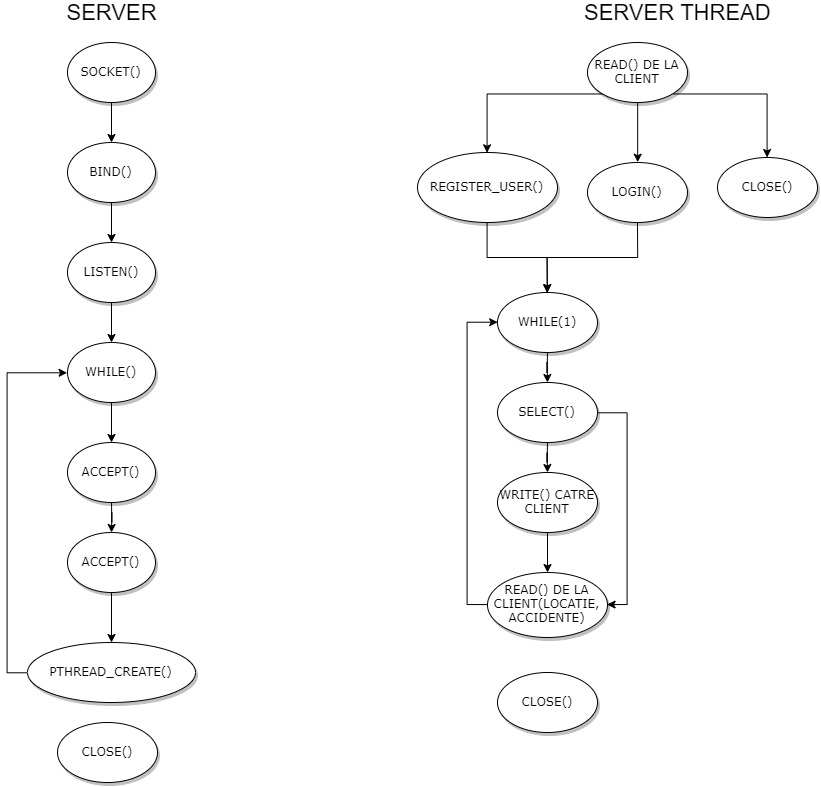
\includegraphics[width=\textwidth]{SERVER_SERVER_THREAD.jpg}
\caption{Diagrama server}
\end{figure}

Clientul va avea un thread si 2 socketi. Pe primul socket va comunica cu serverul datele de logare, si va introduce introduce date in caz de accident. Al doilea socket, va trimite date la server despre locatia si viteza clientului, si va primi de la server informatii despre limita de viteza, incidente (maracte de alti utilizatori) si evenimentele din acea zona.
\begin{figure}[H]
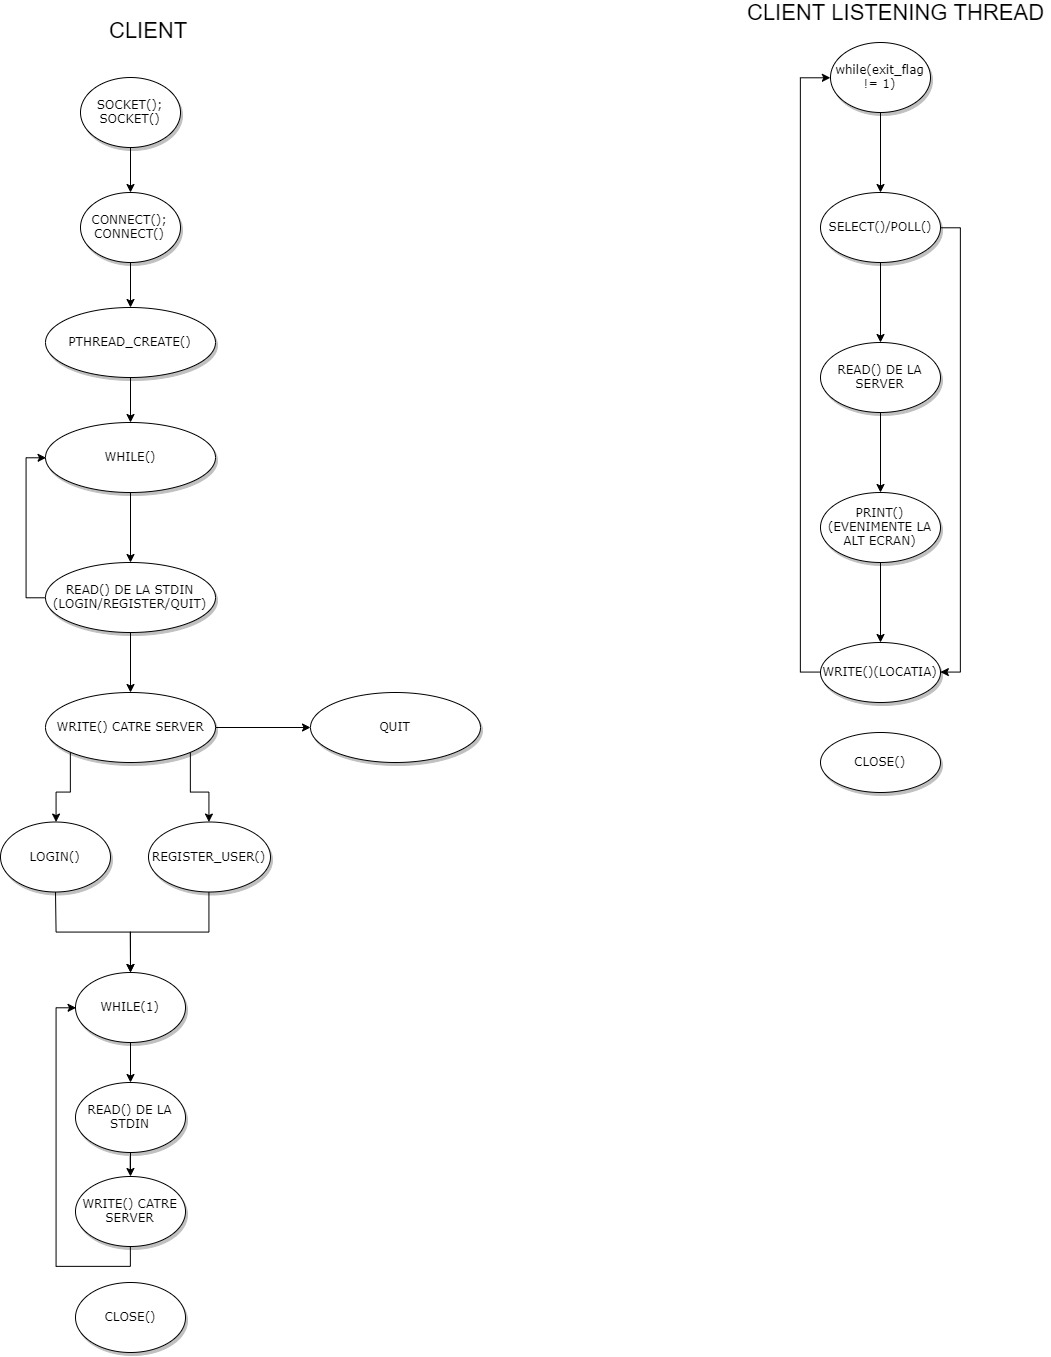
\includegraphics[width=\textwidth]{CLIENT_CLIENT_THREAD.jpg}
\caption{Diagrama client}
\end{figure}
Clientul va avea 2 ecrane diferite, unul in care introduce inputul de la tastatura, si altul care va afisa evenimentele/incidente/limitari de viteza primite de la server in functie de zona in care se afla.\\

Pentru simularea unei harti, voi folosi o matrice, in care fiecare pozitie (linie, coloana) va fi (y, x) intr-un sistem cartezian. Fiecare strada din oras va avea o cate un vector de coordonate (x,y). Reteaua stradala va fi modelata sub forma unui graf, in care muchiile vor fi strazile, iar nodurile vor fi intersectiile. Clientii se vor deplasa de la un punct (x, y) la alt punct (p, q). Pentru a determina un drum de lungime minima, ma voi folosi de un algoritm pentru determinarea unui drum de lungime minima. Zonele cu restrictie de viteza, blocaje si accidente vor fi retinute in server sub forma unor vectori de coordonate.

\begin{figure}[H]
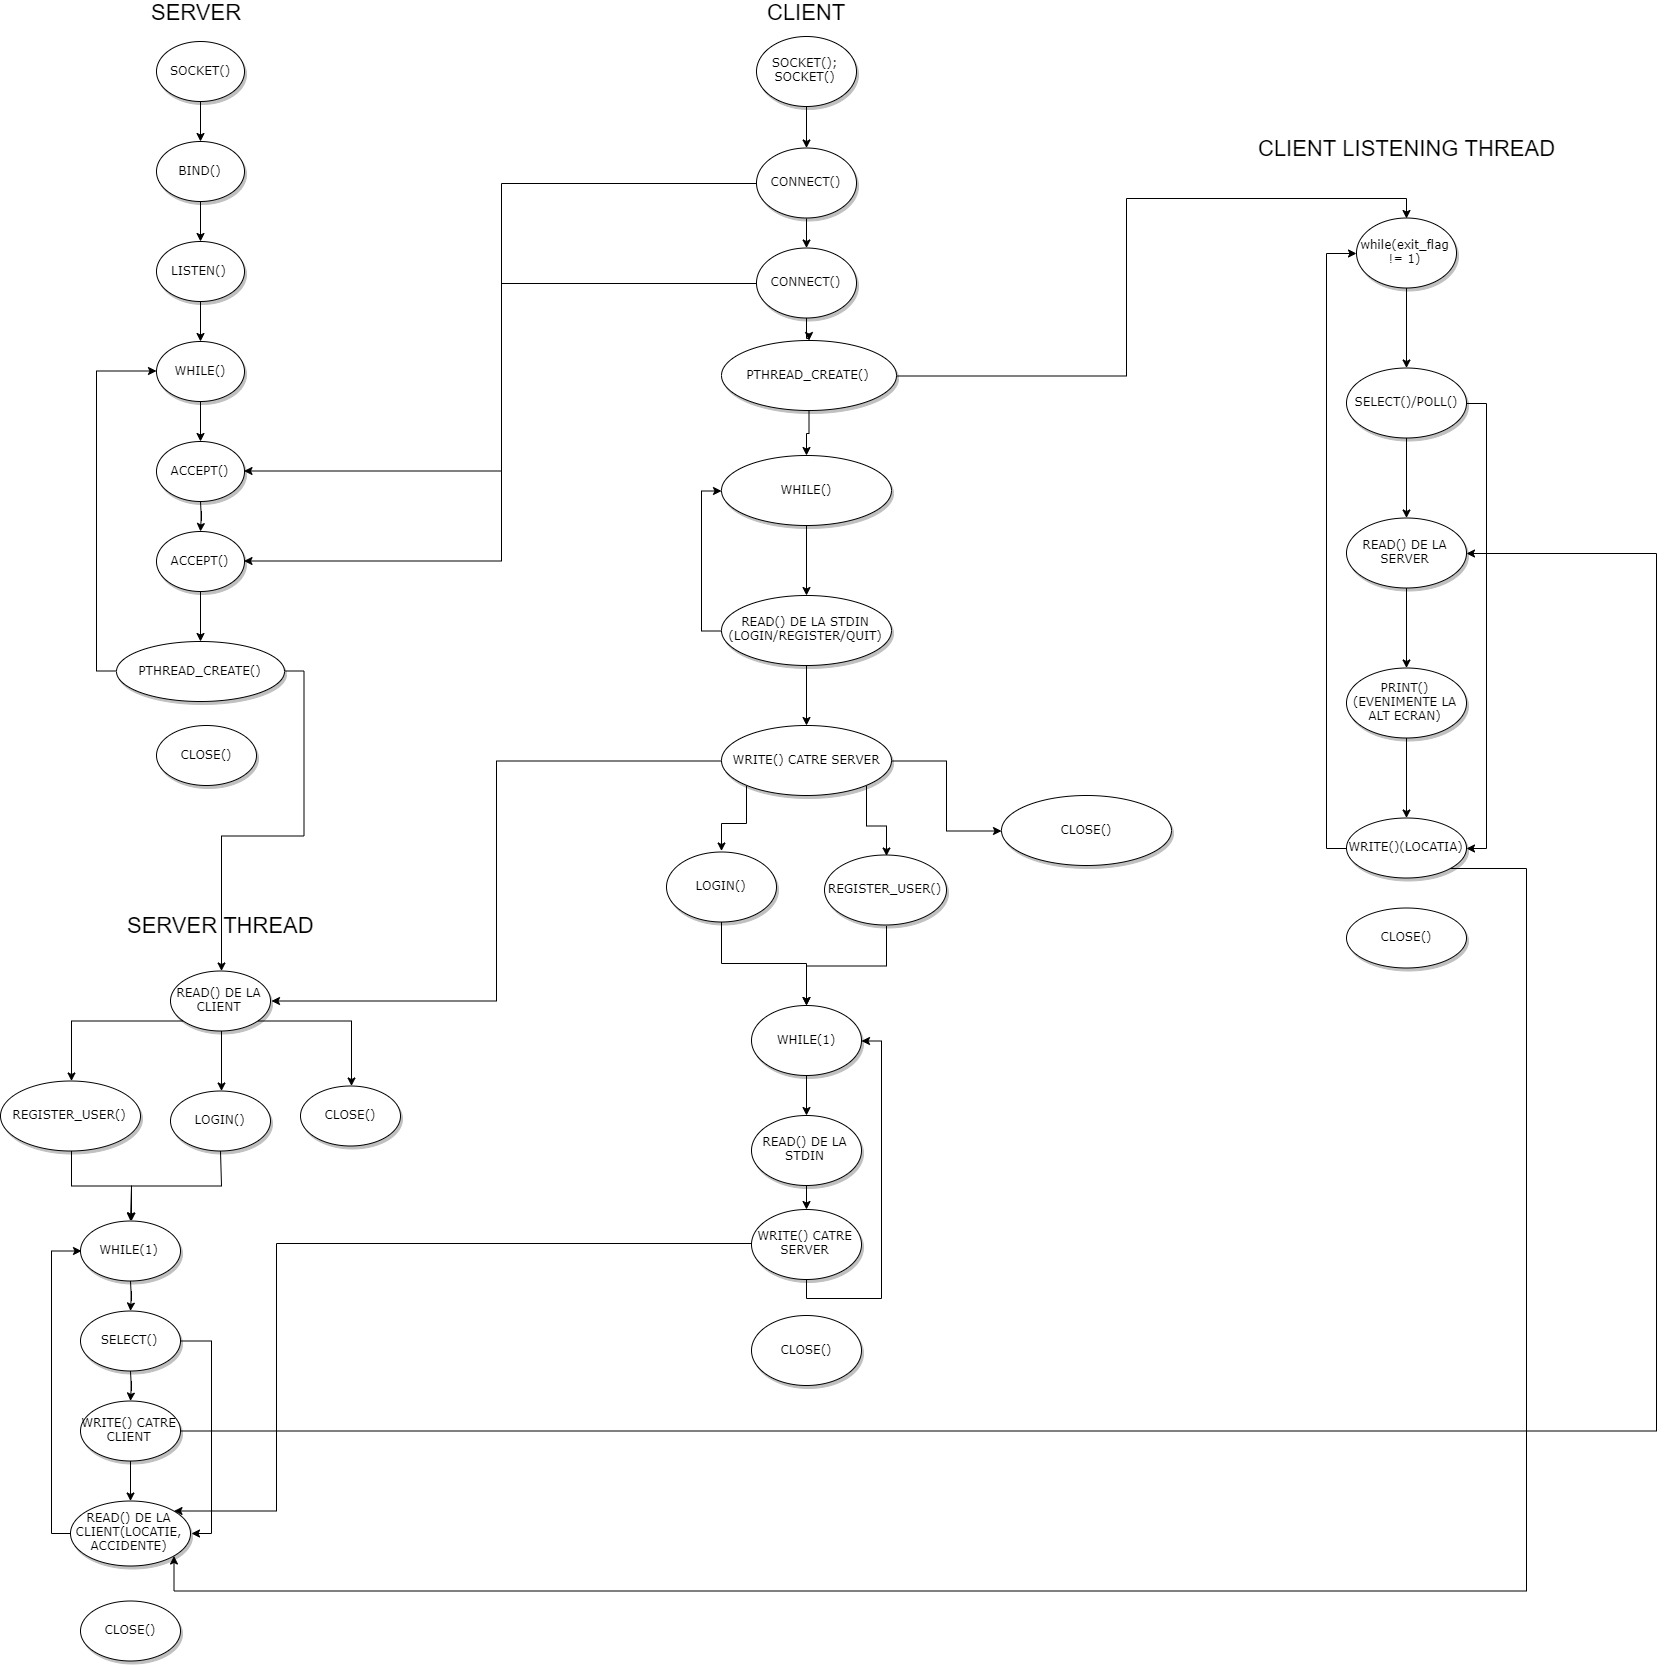
\includegraphics[width=\textwidth]{APPLICATION.jpg}
\caption{Diagrama generala a aplicatiei}
\end{figure}

\begin{figure}[H]
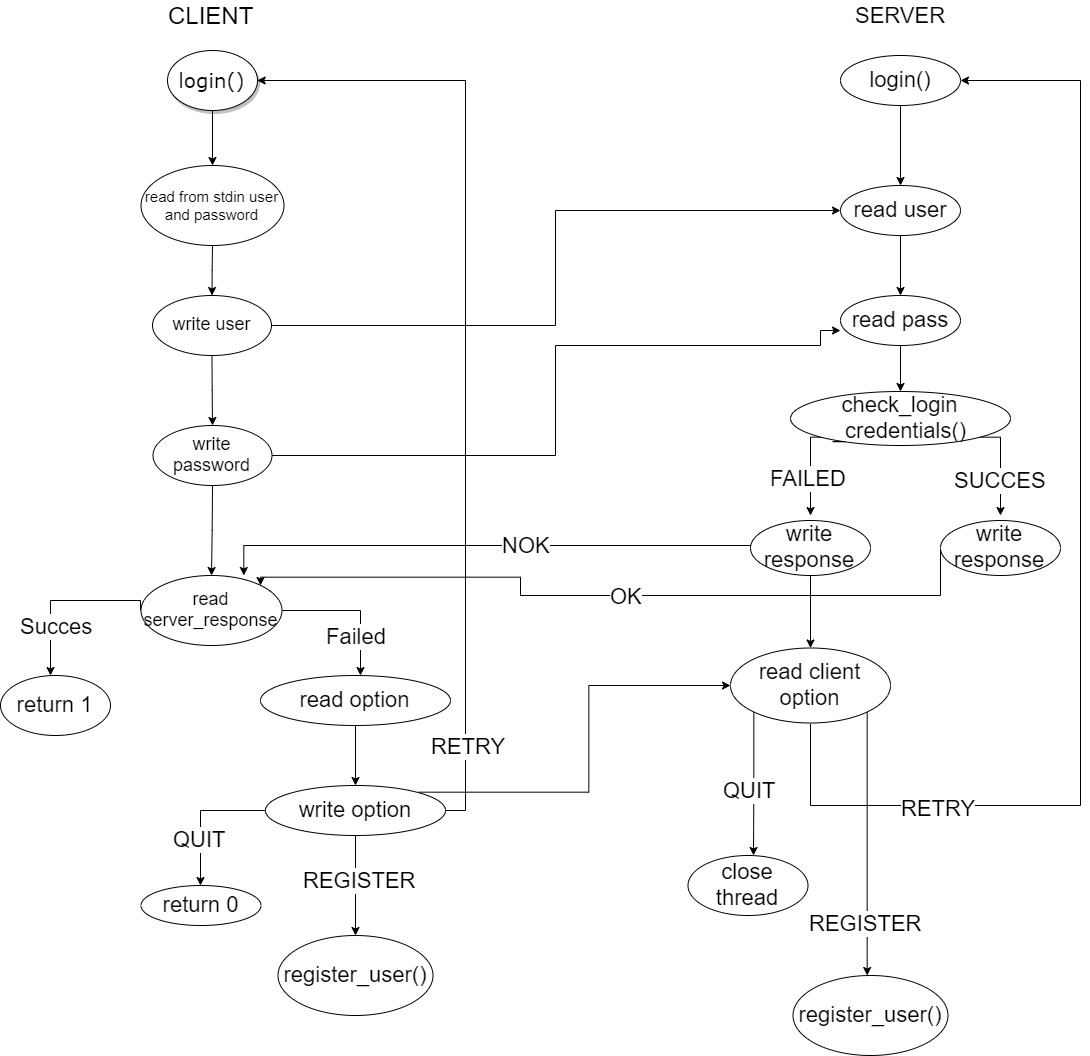
\includegraphics[width=\textwidth]{login.jpg}
\caption{Functia login}
\end{figure}

\begin{figure}[H]
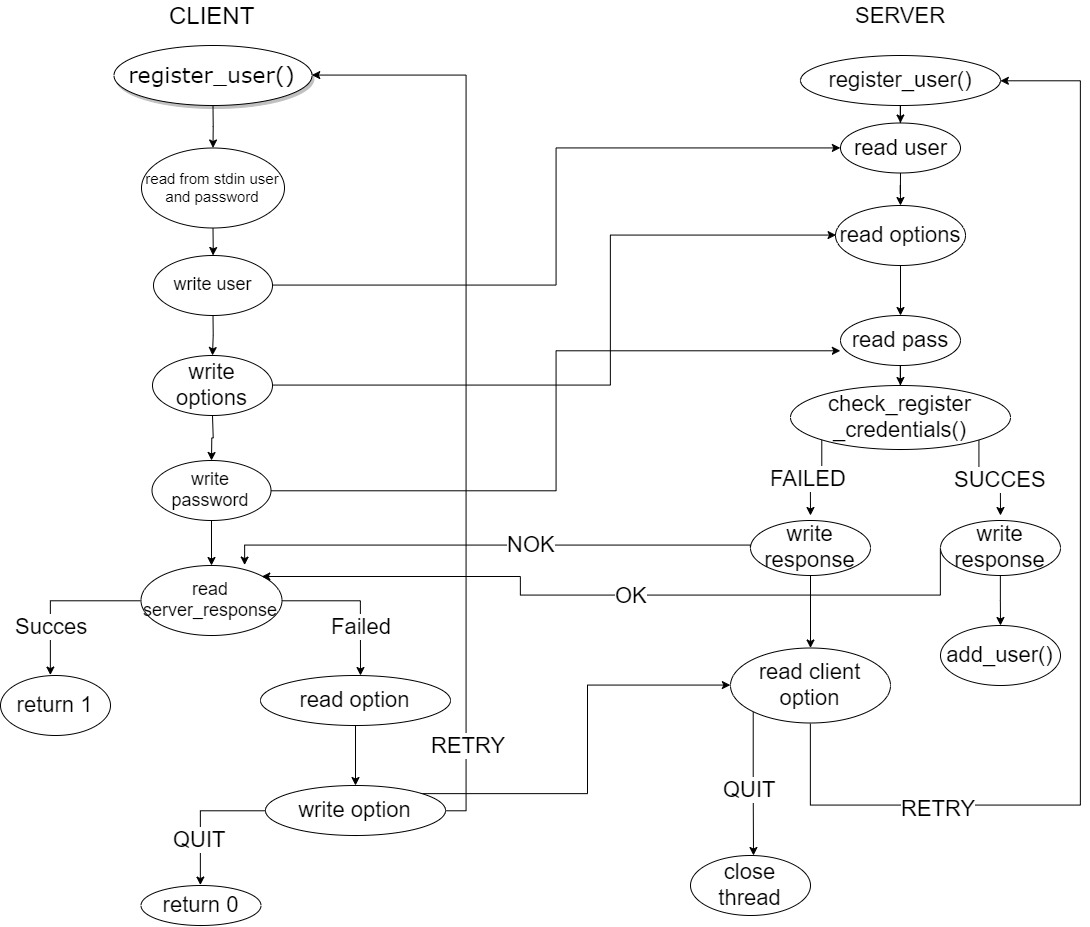
\includegraphics[width=\textwidth]{register.jpg}
\caption{Functia register}
\end{figure}

\section {Detalii de implementare}
Clientul va avea de ales intre register, login si quit. Daca se va inregistra, acesta va trebui sa isi aleaga si evenimentele pe care vrea sa le primeasca(informatii despre vreme, evenimente sportive, preturi pentru combustibili la statiile peco). Dupa ce conectarea s-a realizat cu succes, clientul va putea sa introduca accident sau inchide. Daca introduce accident, va fi intrebat de locatia accidentului si informatia va fi retinuta de server si distribuita catre alti clienti din acea zona.\\
\begin{figure}[H]
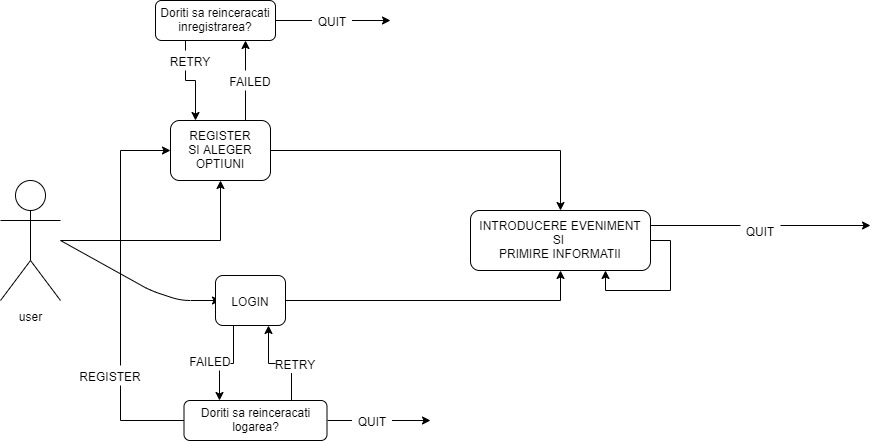
\includegraphics[width=\textwidth]{use-case.jpg}
\caption{Cum va folosi clientul aplicatia}
\end{figure}
Functia de login din client
\begin{lstlisting}
int login(int sd){//1 == succes, 0 == quit
    char* user = (char*)malloc(50);
    char* pass = (char*)malloc(50);
    printf("user : ");
    fgets(user, 50, stdin);
    user[strlen(user) - 1] = '\0';
    printf("\n password : ");
    fgets(pass, 50, stdin);
    pass[strlen(pass) - 1] = '\0';
    if(write(sd, user, 50) < 0){
        perror("Eroare la write");
        return 0;
    }
    if(write(sd, pass, 50) < 0){
        perror("Eroare la write");
        return 0;
    }
    char server_response[100];
    read(sd, server_response, 100);
    if(strcmp(server_response, "OK") == 0){
        printf("\nLOGIN SUCCESFULL\n");
        return 1;
    }else{
        printf("\n Login failed. \n");
        printf("Retry to login or register? Type your option[retry/register/quit] ");
        char * action = (char*)malloc(50);
        fgets(action, 50, stdin);
        action[strlen(action) - 1] = '\0';
        while(strcmp(action, "retry") != 0 && strcmp(action, "quit") != 0 && strcmp(action, "register") != 0 ){
            printf("Please type retry or quit or register.\n");
            fgets(action, 50, stdin);
        }
        if(strcmp(action, "quit") == 0){
            if(write(sd, action, 10) < 0){
                perror("Eroare la write");
                return 0;
            }
            return 0;
        }else if(strcmp(action, "retry") == 0){
            if(write(sd, action, 10) < 0){
                perror("Eroare la write");
                return 0;
            }
            return login(sd);
        }else{
            if(write(sd, action, 10) < 0){
                perror("Eroare la write");
                return 0;
            }
            return register_user(sd);
        }
    }
    return 0;
}
\end{lstlisting}
Functia de register user din client
\begin{lstlisting}
int register_user(int sd){//1 == succes, 0 == quit
    char* user = (char*)malloc(50);
    char* pass = (char*)malloc(50);
    printf(" user : ");
    fgets(user, 50, stdin);
    user[strlen(user) - 1] = '\0';
    printf("\n password : ");
    fgets(pass, 50, stdin);
    pass[strlen(pass) - 1] = '\0';
    if(write(sd, user, 50) < 0){
        perror("Eroare la write");
        return 0;
    }
    if(write(sd, pass, 50) < 0){
        perror("Eroare la write");
        return 0;
    }
    char server_response[100];
    read(sd, server_response, 100);
    if(strcmp(server_response, "OK") == 0){
        printf("\nREGISTER SUCCESFULL\n");
        return 1;
    }else{ // not ok
        printf("\n REGISTER failed. \n");
        printf("Retry to register? Type your option[retry/quit] ");
        char* action = (char*)malloc(50);
        fgets(action, 50, stdin);
        action[strlen(action) - 1] = '\0';
        while(strcmp(action, "retry") != 0 && strcmp(action, "quit") != 0){
            printf("Please type retry or quit \n");
            fgets(action, 50, stdin);
        }
        if(strcmp(action, "quit") == 0){
            if(write(sd, action, 10) < 0){
                perror("Eroare la write");
                return 0;
            }
            return 0;
        }else if(strcmp(action, "retry") == 0){
            if(write(sd, action, 10) < 0){
                perror("Eroare la write");
                return 0;
            }
            return register_user(sd);
        }
    }
    return 0;
}
\end{lstlisting}
Functia register user din server
\begin{lstlisting}
void register_user(int sd, int id){
    /// check ///
    while(1){
        char user[INPUT_SIZE]; 
        char pass[INPUT_SIZE]; 
        read(sd, user, INPUT_SIZE);
        read(sd, pass, INPUT_SIZE);
        int check_code = check_register_credentials(user, pass);
        printf("code = \%d\n", check_code);
        if(check_code == 1){
            write(sd, "NOT OK", 7);
            //vezi ce a trimis clientul
            char option[100];
            read(sd, option, 100);
            if(strcmp(option, "quit") == 0){
                check_code = -1;
                break;
            }else if(strcmp(option, "retry") == 0){
                continue; //bucla while va merge inca o data
            }
        }else if(check_code == 0){//add user
            add_user(user, pass);
            printf("[thread \%d]Clientul \%s s-a inregistrat cu succes!\n", id, user);
            write(sd, "OK", 3);
            break;             
        }
    }
}
\end{lstlisting}
Functia check login credentials din server
\begin{lstlisting}
int check_login_credentials(char*user, char*pass){// -1 daca e eroare, 1 daca am gasit user + pass, 0 altfel
    int fd = open("useri.txt", O_RDWR);
    if(fd < 0){
        perror("Eroare la deschidere fisier");
        return -1;
    }
    int found = 0, k = 0;
    char word1[110];
    while(!found){//parcurg fisierul
        unsigned char ch;
        int codr = read(fd, &ch, 1);
        if(codr == 0){  //end of file
            break;
        }else if(codr == -1){
            perror("Eroare la citire");
            close(fd);
            return -1;
        }
        if(ch != ' ' && ch != '\n'){//obtinem user-ul de pe o linie
            word1[k++] = ch;
        }
        if(ch == ' '){
            word1[k] = '\0';
            
            if(strcmp(word1, user) != 0){//daca e un user diferit, sarim linia
                while(ch != '\n'){//parcurgem linia pana la sfarsit
                    read(fd, &ch, 1);
                }
                k = 0;
            }else{ // daca am gasit user-ul verificam parola
                int t = 0;
                char password[50];
                
                while(ch != '\n'){//obtinem parola
                    read(fd, &ch, 1);
                    password[t++] = ch;
                }
                password[t-1] = '\0';
                
                if(strcmp(pass, password) == 0){//verificam parola
                    close(fd);
                    return 1;
                }
                k = 0;
            }
        }
    }
    close(fd);
    return found;
}
\end{lstlisting}

Un thread din server
\begin{lstlisting}
void* routine(void*arg){
    thData thread = *((thData*)arg);
    printf("[thread \%d] Vom comunica cu clientul cu fd \%d\n", thread.thread_id, thread.client_fd);
    int client_fd = thread.client_fd;
    char client_option[100];
    read(client_fd, client_option, 100);
    printf("[thread \%d]Am primit >\%s< de la client\n", thread.thread_id, client_option);
    if(strcmp(client_option, "register") == 0){
        register_user(client_fd, thread.thread_id);
    }else if(strcmp(client_option, "login") == 0){
        login(client_fd, thread.thread_id);
    }else if(strcmp(client_option, "quit") == 0){
        printf("[thread \%d] Inchidere thread.\n", thread.thread_id);
        close((uintptr_t)arg);
        return NULL;
    }
    //TODO: broadcast cu thread.broadcast_fd
    printf("[thread \%d]Inchidem thread.\n", thread.thread_id);
    close((uintptr_t)arg);
    return NULL;
}
\end{lstlisting}

\section {Concluzii}

Acest proiect poate fi imbunatatit prin implementarea unei interfete grafice care sa afiseze o harta actualizata in timp real. De asemenea, daca s-ar putea modifica optiunile alese de clienti si dupa ce s-au inregistrat, utilizatorii ar avea parte de o experienta mai buna a aplicatiei.\\

Pentru a imbunatati viteza serverului, as putea sa apelez functia accept() in threaduri, adica sa fac un threadpoll, sau as putea sa implementez un server TCP prethreaded.
\\
\\
\section {Bibliografie}
\begin{thebibliography}{8}
\bibitem{ref_url1}
\url{https://www.tutorialspoint.com/sqlite/sqlite\_c\_cpp.htm}
\bibitem{ref_url1}
\url{https://www.sqlite.org/cintro.html}
\bibitem{ref_url1}
\url{https://www.sqlite.org/cintro.html}
\bibitem{ref_url1}
\url{https://profs.info.uaic.ro/~computernetworks/files/NetEx/S12/ServerConcThread/servTcpConcTh2.c}
\bibitem{ref_url1}
\url{https://profs.info.uaic.ro/~computernetworks/files/NetEx/S12/ServerConcThread/cliTcpNr.c}
\bibitem{ref_url1}
\url{https://profs.info.uaic.ro/~computernetworks/files/7rc\_ProgramareaInReteaIII\_Ro.pdf}
\bibitem{ref_url1}
\url{https://www.qt.io/}
\bibitem{ref_url1}
\url{https://glade.gnome.org/}
\bibitem{ref_url1}
\url{https://profs.info.uaic.ro/~computernetworks/cursullaboratorul.php}

\end{thebibliography}

\end{document}


